
% This LaTeX was auto-generated from MATLAB code.
% To make changes, update the MATLAB code and republish this document.

\documentclass{article}
\usepackage{graphicx}
\usepackage{color}

\sloppy
\definecolor{lightgray}{gray}{0.5}
\setlength{\parindent}{0pt}

\begin{document}

    
    \begin{verbatim}
clear; clc

% params
theta0 = 0.01;
w0 = 0;
m1 = 2;
m2 = 1;
g = 10;
L = 0.75;
T = 1.5;

xinitial = [theta0,0,w0,0];

t = 0:0.01:T;
u = ones(size(t));

% nonlinear model
G = @(t,x) [x(2);
    g*(m1+m2)*sin(x(1))/(L*(m1+m2*sin(x(1)).^2))-0.5*m2*sin(2*x(1))*x(2).^2/(m1+m2*sin(x(1)).^2);
    x(4);
    -L*m2*sin(x(1))*x(2).^2/(m1+m2*sin(x(1)).^2)+0.5*g*m2*sin(2*x(1))/(m1+m2*sin(x(1)).^2)] + [0;cos(x(1))/(L*(m1+m2*sin(x(1)).^2));0;1/(m1+m2*sin(x(1)).^2)];

[tnonlinear,xnonlinear] = ode45(G,[0,T],xinitial);

thetanonlinear = xnonlinear(:,1);
wnonlinear = xnonlinear(:,3);

% linear model
A = [0 1 0 0;g*(m1+m2)/(m1*L) 0 0 0;0 0 0 1;g*m2/m1 0 0 0];
B = [0;1/(L*m1);0;1/m1];
D = 0;

sysw = ss(A,B,[0 0 1 0],D);
wlinear = lsim(sysw,u,t,xinitial);

syst = ss(A,B,[1 0 0 0],D);
thetalinear = lsim(syst,u,t,xinitial);


% cart position plot
figure, hold on
plot(tnonlinear,wnonlinear,'r-','DisplayName','Non-linear state space')
plot(t,wlinear,'b-','DisplayName','Linear state space')
legend('show')
xlabel('t [s]')
ylabel('w(t) [m]')

ha = gca;
box on
grid on
set(ha,'GridLineStyle','--')
print(gcf,'fig3.png','-dpng','-r500');


% pendulum position plot
figure, hold on
plot(tnonlinear,thetanonlinear,'r-','DisplayName','Non-linear state space')
plot(t,thetalinear,'b-','DisplayName','Linear state space')
legend('show')
xlabel('t [s]')
ylabel('\theta(t) [rad]')

ha = gca;
box on
grid on
set(ha,'GridLineStyle','--')
print(gcf,'fig4.png','-dpng','-r500');

hold off
\end{verbatim}

\includegraphics [width=4in]{step_ssmodel_01.eps}

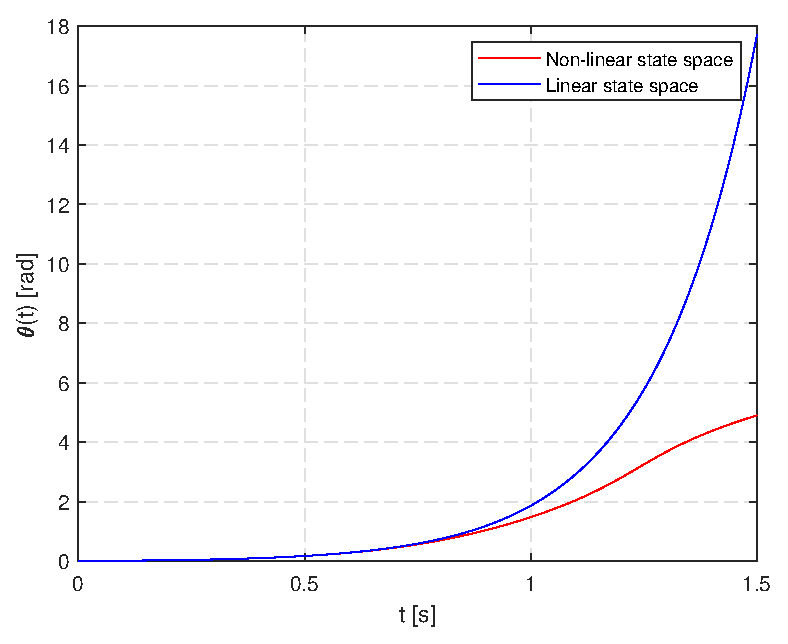
\includegraphics [width=4in]{step_ssmodel_02.eps}



\end{document}

